% --------------------------------------------------------------
%                           Set Up
% --------------------------------------------------------------
 
\documentclass[12pt]{article}
 
\usepackage[margin=1in]{geometry} 
\usepackage{amsmath,amsthm,amssymb}
\usepackage{listings}
\usepackage{xcolor}
\usepackage{graphicx}
\usepackage{subcaption}
\usepackage{listings}
\usepackage{xcolor}
\usepackage{comment}
\usepackage{hepnames}
\usepackage{longtable}
 
\definecolor{codegreen}{rgb}{0,0.6,0}
\definecolor{codegray}{rgb}{0.5,0.5,0.5}
\definecolor{codepurple}{rgb}{0.58,0,0.82}
\definecolor{backcolour}{rgb}{0.95,0.95,0.92}
 
\lstdefinestyle{mystyle}{
    backgroundcolor=\color{backcolour},   
    commentstyle=\color{codegreen},
    keywordstyle=\color{magenta},
    numberstyle=\tiny\color{codegray},
    stringstyle=\color{codepurple},
    basicstyle=\ttfamily\footnotesize,
    breakatwhitespace=false,         
    breaklines=true,                 
    captionpos=b,                    
    keepspaces=true,                 
    numbers=left,                    
    numbersep=5pt,                  
    showspaces=false,                
    showstringspaces=false,
    showtabs=false,                  
    tabsize=2
}
 
\lstset{style=mystyle}
 
\definecolor{codegreen}{rgb}{0,0.6,0}
\definecolor{codegray}{rgb}{0.5,0.5,0.5}
\definecolor{codepurple}{rgb}{0.58,0,0.82}
\definecolor{backcolour}{rgb}{0.95,0.95,0.92}
\definecolor{deepblue}{rgb}{0,0,0.5}
\definecolor{deepred}{rgb}{0.6,0,0}
\definecolor{deepgreen}{rgb}{0,0.5,0}
 
\lstdefinestyle{mystyle}{
    backgroundcolor=\color{backcolour},   
    commentstyle=\color{codegreen},
    keywordstyle=\color{deepred},
    numberstyle=\tiny\color{codegray},
    stringstyle=\color{deepblue},
    basicstyle=\ttfamily\footnotesize,
    breakatwhitespace=false,         
    breaklines=true,                 
    captionpos=b,                    
    keepspaces=true,                 
    numbers=left,                    
    numbersep=5pt,                  
    showspaces=false,                
    showstringspaces=false,
    showtabs=false,                  
    tabsize=2
}
 
\lstset{style=mystyle}
 
\newcommand{\N}{\mathbb{N}}
\newcommand{\Z}{\mathbb{Z}}
 
\newenvironment{theorem}[2][Theorem]{\begin{trivlist}
\item[\hskip \labelsep {\bfseries #1}\hskip \labelsep {\bfseries #2.}]}{\end{trivlist}}
\newenvironment{lemma}[2][Lemma]{\begin{trivlist}
\item[\hskip \labelsep {\bfseries #1}\hskip \labelsep {\bfseries #2.}]}{\end{trivlist}}
\newenvironment{exercise}[2][Exercise]{\begin{trivlist}
\item[\hskip \labelsep {\bfseries #1}\hskip \labelsep {\bfseries #2.}]}{\end{trivlist}}
\newenvironment{problem}[2][Problem]{\begin{trivlist}
\item[\hskip \labelsep {\bfseries #1}\hskip \labelsep {\bfseries #2.}]}{\end{trivlist}}
\newenvironment{question}[2][Question]{\begin{trivlist}
\item[\hskip \labelsep {\bfseries #1}\hskip \labelsep {\bfseries #2.}]}{\end{trivlist}}
\newenvironment{corollary}[2][Corollary]{\begin{trivlist}
\item[\hskip \labelsep {\bfseries #1}\hskip \labelsep {\bfseries #2.}]}{\end{trivlist}}

\newenvironment{solution}{\begin{proof}[Solution]}{\end{proof}}

\setlength\parindent{0pt}
 
\begin{document}
 
% -------------------------------------------------------------- 
%                         Start here
% --------------------------------------------------------------
 
\title{Homework 5}
\author{Timothy Holmes\\ %replace with your name
PHY 442 Computational Physics}

\maketitle

\section*{Problem 1}

The five images below are produced using the Fourier Series code in the appendix. Figures 1(a), 1(b), 1(d), and 1(e) are very similar. It can be seen that as $n$ increases, the function smooths out. A strange difference in Figure 1(c) occurs when n = 30. However, this smoothing affect is the Gibbs phenomena. 


\begin{figure}[h!]
\centering

\begin{subfigure}{0.49\columnwidth}
\centering
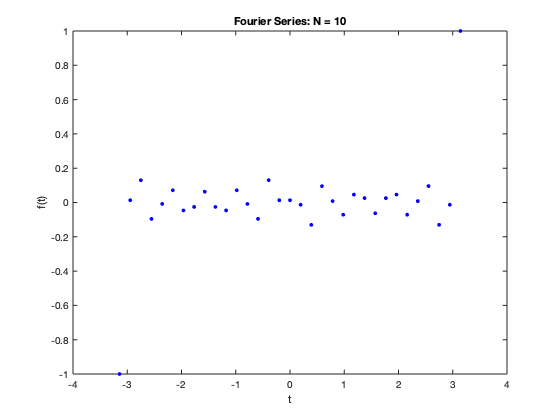
\includegraphics[width=\textwidth]{fs_n_10.png}
\caption{}
\label{fig:time1}
\end{subfigure}\hfill
\begin{subfigure}{0.49\columnwidth}
\centering
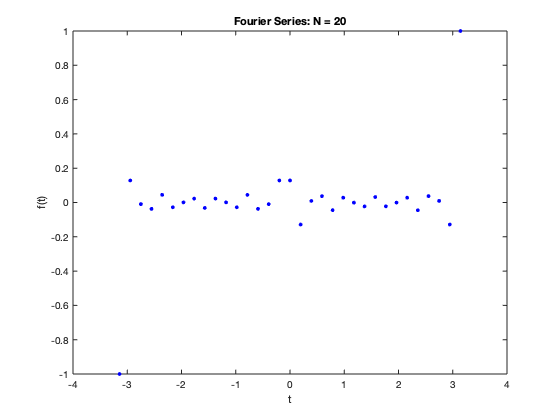
\includegraphics[width=\textwidth]{fs_n_20.png}
\caption{}
\label{fig:time2}
\end{subfigure}

\medskip

\begin{subfigure}{0.49\columnwidth}
\centering
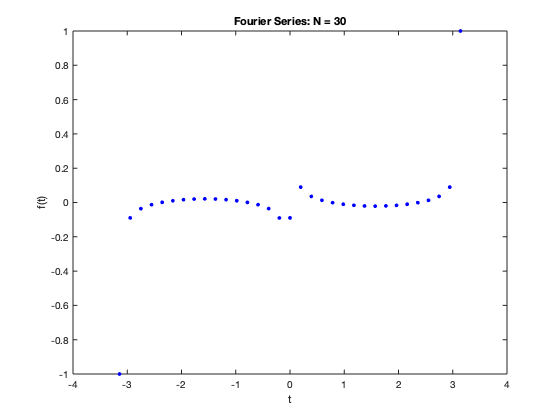
\includegraphics[width=\textwidth]{fs_n_30.png}
\caption{}
\label{fig:time3}
\end{subfigure}\hfill
\begin{subfigure}{0.49\columnwidth}
\centering
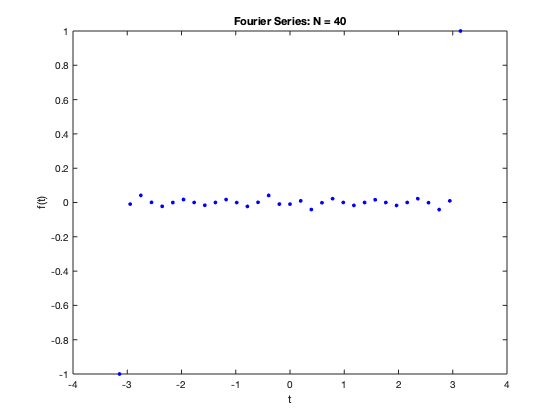
\includegraphics[width=\textwidth]{fs_n_40.png}
\caption{}
\label{fig:time4}
\end{subfigure}

\medskip

\begin{subfigure}{0.49\columnwidth}
\centering
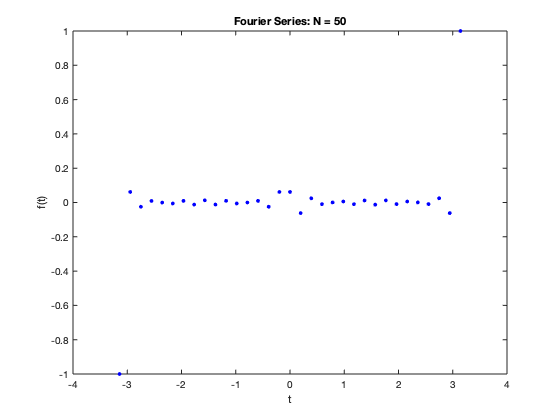
\includegraphics[width=\textwidth]{fs_n_50.png}
\caption{}
\label{fig:time5}
\end{subfigure}

\caption{Various plots from $n = 10$ to $n = 50$.}
\label{fig:time}

\end{figure}

\newpage



\newpage


\newpage

\section*{Problem 2}

The numerical Fourier Transform produces the image below. The code to procure this can be found in the appendix.

\begin{figure}[h!]
    \centering
    {{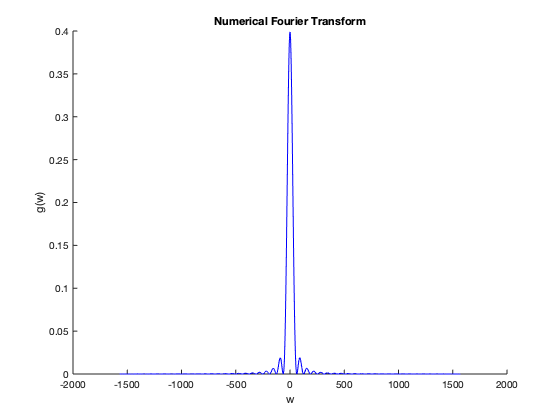
\includegraphics[width=15cm]{numerical_ft.png}}}%
    \qquad
    \caption{ }%
    \label{fig:example}%
\end{figure}

\newpage

\section*{Problem 3}

The Discrete Fourier Transform produces the image below. The code to procure this can be found in the appendix. Unlike the numerical version this method does not plot a max value at $\omega = 0$.


\begin{figure}[h!]
    \centering
    {{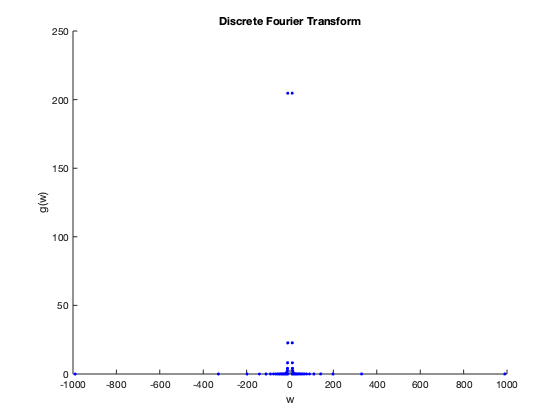
\includegraphics[width=15cm]{DFT.png}}}%
    \qquad
    \caption{ }%
    \label{fig:example}%
\end{figure}

\newpage

\section*{Problem 4}

The Fast Fourier Transform produces the image below. The code to procure this can be found in the appendix. Unlike the numerical version this method does not plot a max value at $\omega = 0$. This result is similar to the Discrete Fourier Transform.

\begin{figure}[h!]
    \centering
    {{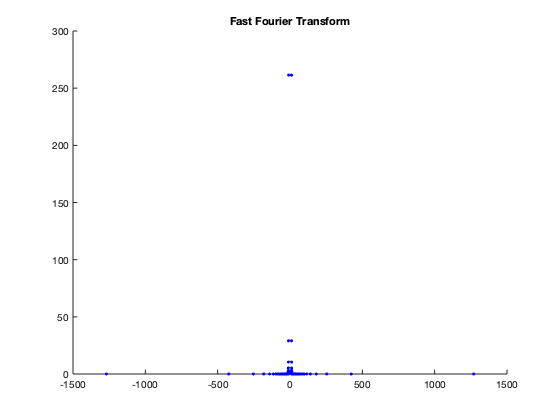
\includegraphics[width=15cm]{FFT.png}}}%
    \qquad
    \caption{ }%
    \label{fig:example}%
\end{figure}

\newpage

\section*{Problem 5}

have not done enough
not far enough starting to see a similar shape, getting a duel shape
middle upper and lower
and final get proper rate

The plot of the real function is the figure below. But this does not tell us much about sampling. 

\begin{figure}[h!]
    \centering
    {{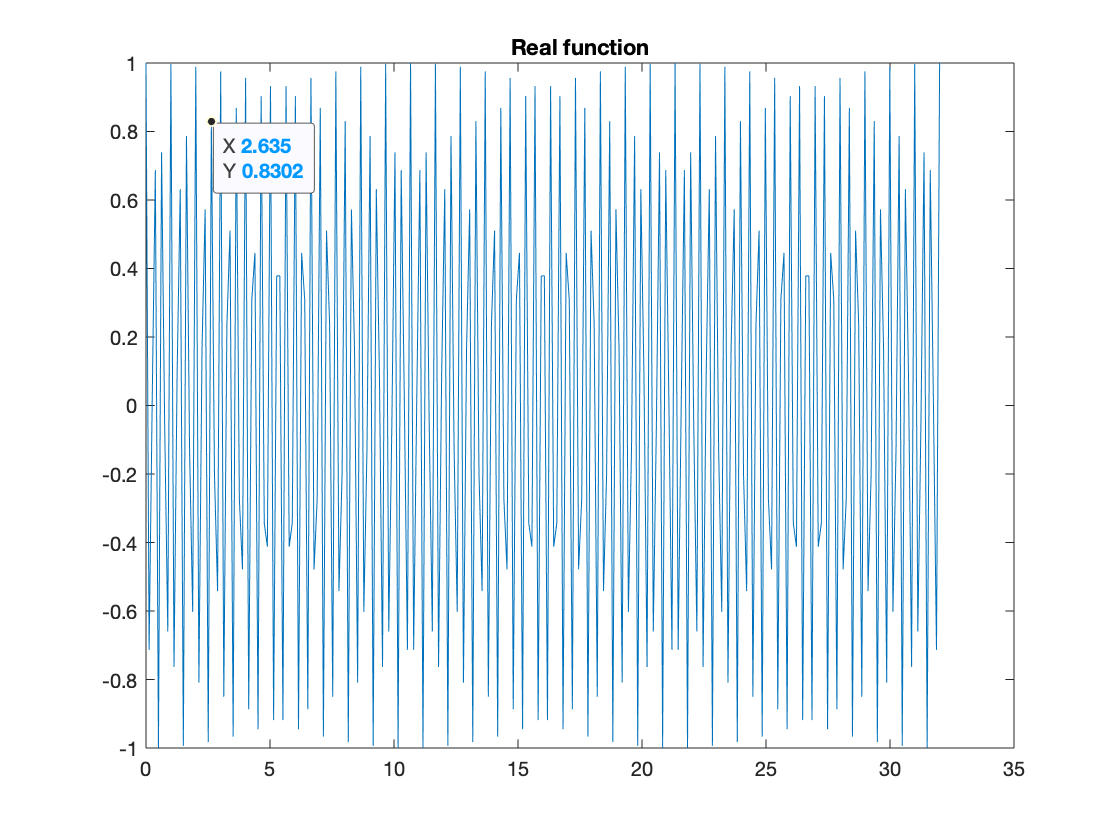
\includegraphics[width=15cm]{problem_5.png}}}%
    \qquad
    \caption{ }%
    \label{fig:example}%
\end{figure}


\begin{figure}[h!]
\centering

\begin{subfigure}{0.49\columnwidth}
\centering
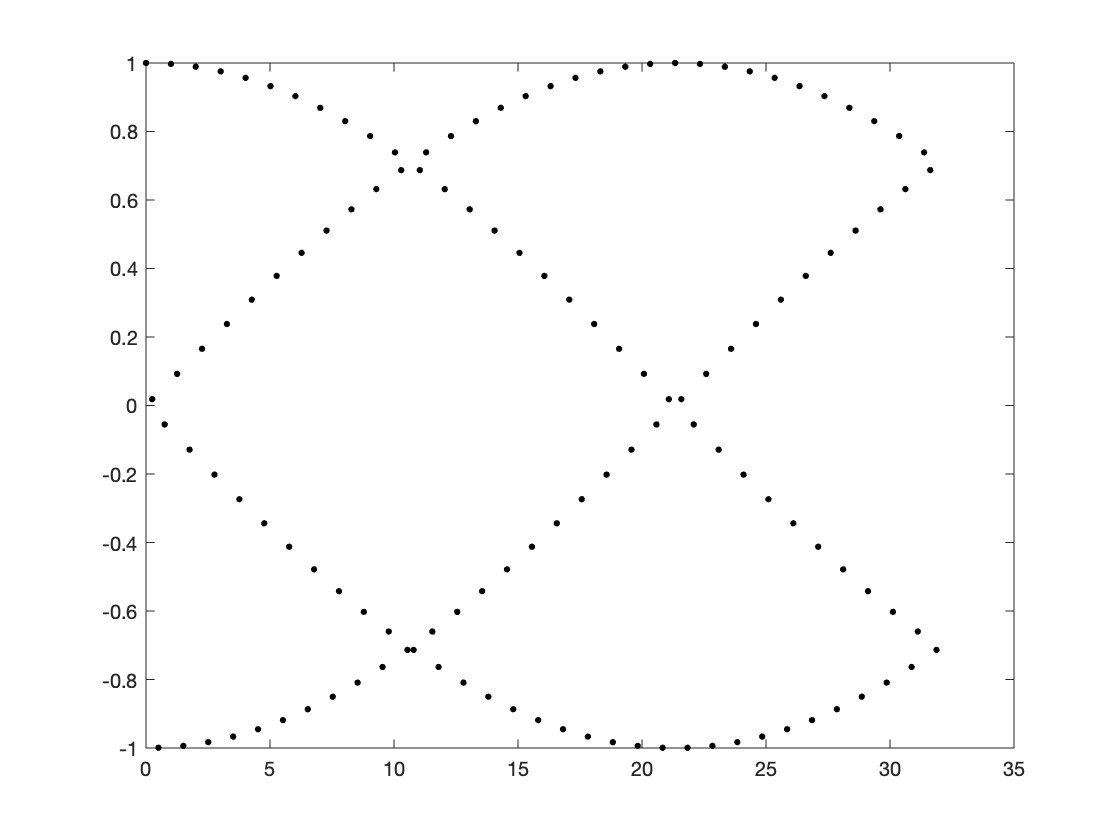
\includegraphics[width=\textwidth]{problem_5_1.png}
\caption{}
\label{fig:time1}
\end{subfigure}\hfill
\begin{subfigure}{0.49\columnwidth}
\centering
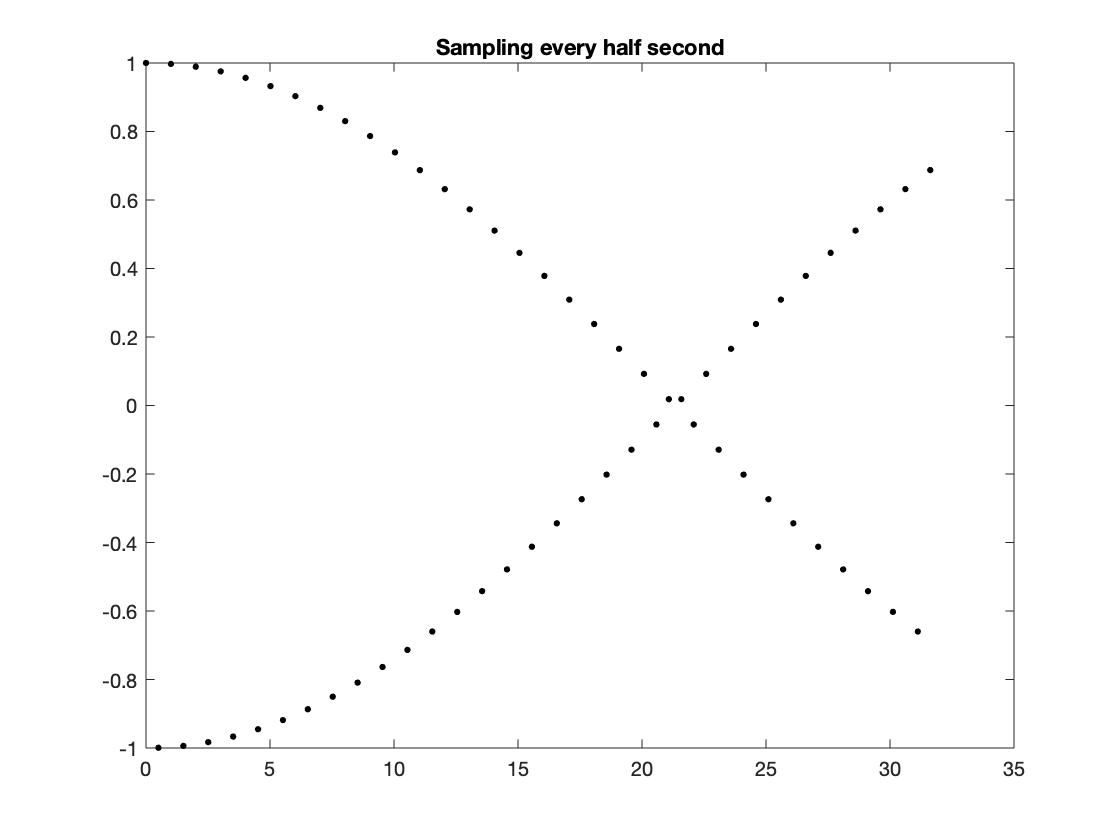
\includegraphics[width=\textwidth]{problem_5_2.png}
\caption{}
\label{fig:time2}
\end{subfigure}

\medskip

\begin{subfigure}{0.49\columnwidth}
\centering
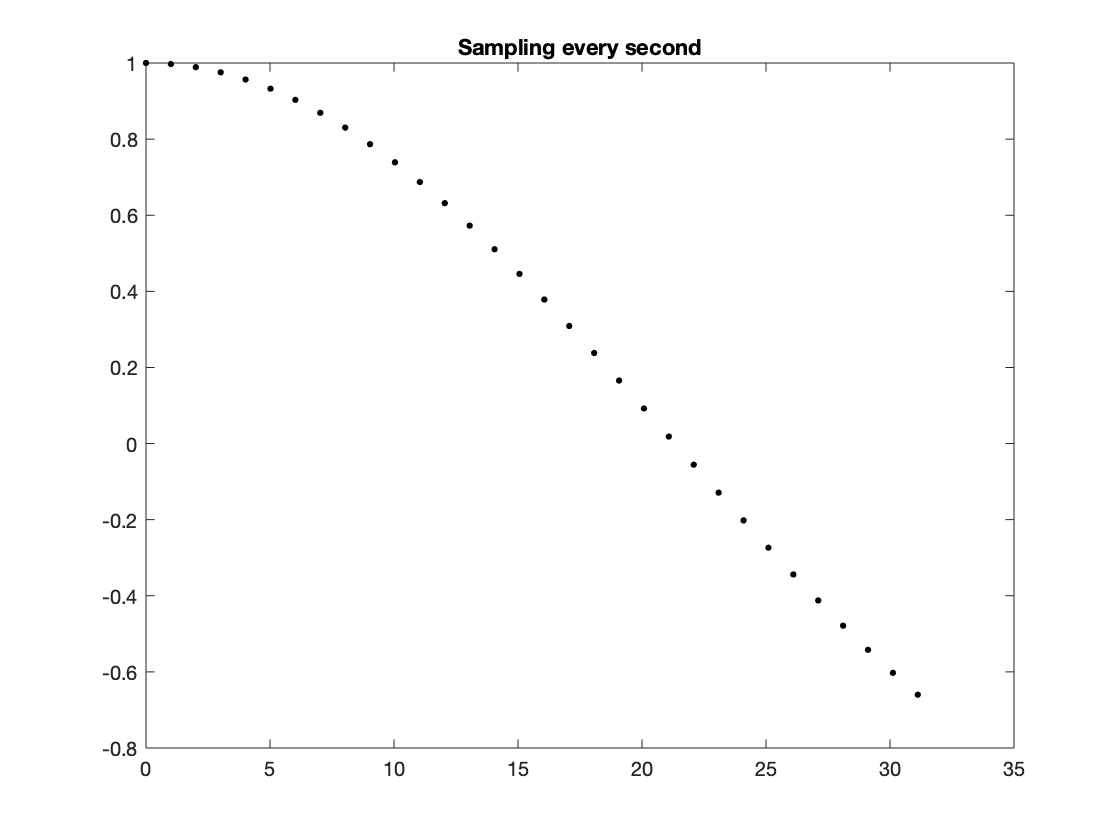
\includegraphics[width=\textwidth]{problem_5_3.png}
\caption{}
\label{fig:time3}
\end{subfigure}\hfill

\caption{Various sample plots.}
\label{fig:time}

\end{figure}

Figure 1(a) has a middle plot that is doubled as well as an upper and lower plot. Figure 1(b) also has a similar feature where it has an upper and lower plot to it. These plots have been over sampled but we get a unique shape out of all of these plots. The final plot has a unique shape we see in all of the previous figures when the sample rate is every second. This is the correct sample rate for the function.

\newpage

\section*{Problem 6}

The plot of the real function is the figure below. 

\begin{figure}[h!]
    \centering
    {{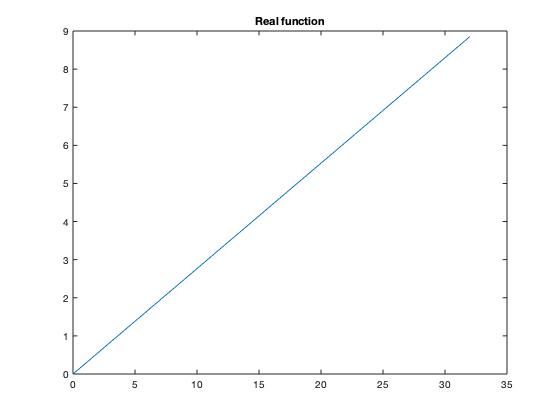
\includegraphics[width=15cm]{problem_6.png}}}%
    \qquad
    \caption{ }%
    \label{fig:example}%
\end{figure}

This problem was very similar to problem 5 in essence. The real look of this function just happens to be a linear line and when $\alpha$ gets to the values of 0.7-0.8 the function behaves a little different by having a negative slope instead of a positive slope. Furthermore, changing the $N$ values did not have any noticeable difference other than for making the time longer and showing more of a linear line. Images from the samples are shown below.

\begin{figure}[h!]
\centering

\begin{subfigure}{0.49\columnwidth}
\centering
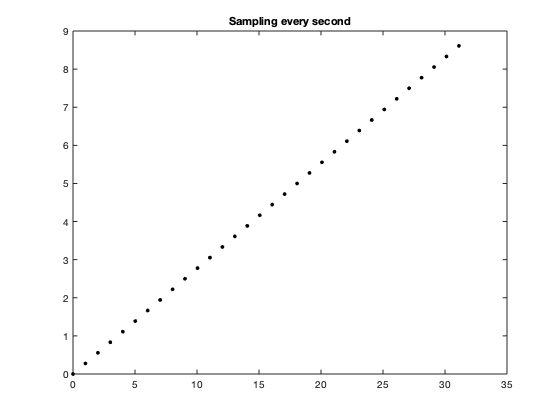
\includegraphics[width=\textwidth]{problem_6_1.png}
\caption{}
\label{fig:time1}
\end{subfigure}\hfill
\begin{subfigure}{0.49\columnwidth}
\centering
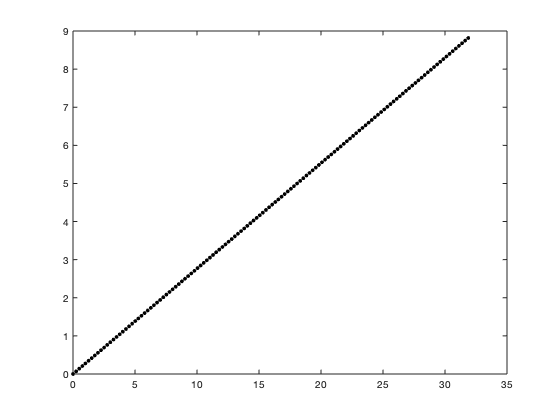
\includegraphics[width=\textwidth]{problem_6_2.png}
\caption{}
\label{fig:time2}
\end{subfigure}

\medskip

\begin{subfigure}{0.49\columnwidth}
\centering
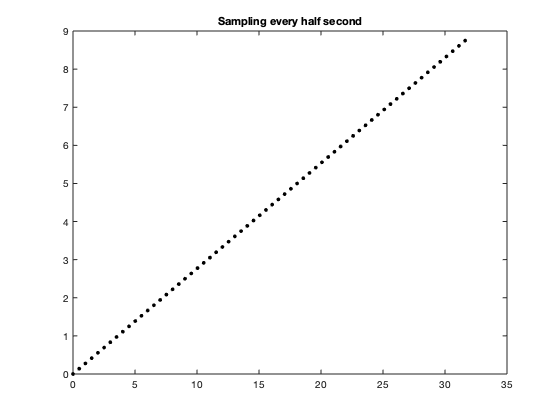
\includegraphics[width=\textwidth]{problem_6_3.png}
\caption{}
\label{fig:time3}
\end{subfigure}\hfill

\caption{Various sample plots.}
\label{fig:time}

\end{figure}

\newpage

\newpage

\section*{Problem 7}

Given a stream of data $v_{out}(t)$, this can be processed by a FFT function that process that data such that the output is $F(v_{out}(t)$. To find $v_{in}$ one last piece of information is needed. The response function for an RC Circuit is 

$$
\frac{1}{RC}e^{-t/RC}
$$

when $t \ge 0$ or $0$ otherwise. In this problem both $R$ and $C$ hold a value of $1$ for simplicity. Given this array of data, the FFT is taken again such that $r(t)$ becomes $F(r(t))$. $v_{in}(t)$ is gave by

$$
V_{in}(t) = F^{-1}\Bigg[ \frac{F(V_{out}(t))}{F(r(t))}\Bigg]
$$

therefore dividing $F(v_{out}(t)$ by $F(r(t))$ and taking the inverse FFT will give the results for $V_{in}(t)$. $\omega$ can be found by $\omega = 1/t$ which is just a frequency. Plotting the frequency by $V_{in}(t)$ results int he following figure.

\begin{figure}[h!]
    \centering
    {{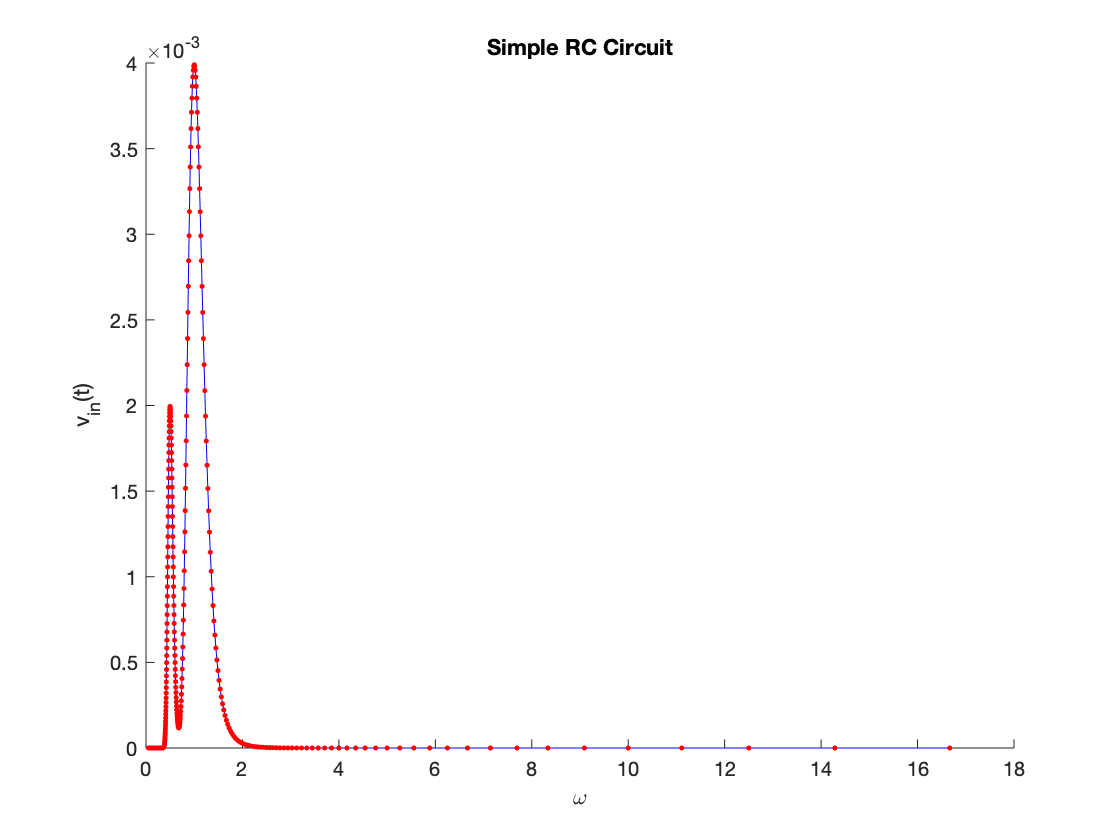
\includegraphics[width=15cm]{v_in.png}}}%
    \qquad
    \caption{ }%
    \label{fig:example}%
\end{figure}

\newpage

\section*{Problem 8}

The figure below shows the output of the tuning fork data. The frequency can be found at $4325$ on the plot.

\begin{figure}[h!]
    \centering
    {{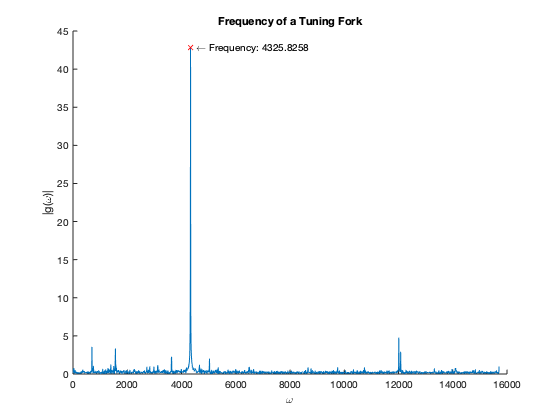
\includegraphics[width=15cm]{tuning_fork.png}}}%
    \qquad
    \caption{ }%
    \label{fig:example}%
\end{figure}

\newpage

\section*{Appendix}

\subsection*{Homework 5 Main Function}
\begin{lstlisting}[language=Matlab, caption= ]
function homework_5()

    fprintf('Enter an integer for what problem you want to run 1-8\n')
    prompt = input('What problem do you want to run? \n problem: ');


    if prompt == 1
        problem_1()

    elseif prompt == 2
        problem_2()

    elseif prompt == 3
        problem_3()

    elseif prompt == 4
        problem_4()

    elseif prompt == 5
        problem_5()

    elseif prompt == 6
        problem_6()

    elseif prompt == 7
        problem_7()

    elseif prompt == 8
        problem_8()

    end

end

function problem_1()

    t0   = -pi;
    tf   = pi;
    step = pi/16; 
    nmax = [10, 20, 30, 40, 50];

    for i = 1:length(nmax)
        fourier_series(t0, tf, step, nmax(i))
        pause()
        clf;
    end

    close;

end

function problem_2()

    a = 10;
    T = 2/a;
    N = 5000;
    n = linspace(-100, 100, N);
    omega = n * pi/T;
    g_w = zeros(N, 1);

    for j = 1:N

        f_t = @(t, a) (a * (1 - a * abs(t)));

        g_w(j) = 1/sqrt(2 * pi) * integral(@(t) f_t(t, a) ...
                 .* exp(-1 * 1i * omega(j) * t), -1/a, 1/a, ... 
                 'RelTol', 0, 'AbsTol', 1e-5);
    end

    figure(1)
    hold on
    title('Numerical Fourier Transform')
    plot(omega, abs(g_w), 'b')
    xlabel('w')
    ylabel('g(w)')

end

function problem_3()

    N = 100;
    a = 10;
    t = linspace(-1/a, 1/a, N);
    omega = 1./t;
    f_t = (a * (1 - a * abs(t)));

    g_w = zeros(N,1);
    for n = 0:N - 1
        g_w(n + 1) = 0;
        for m = 0:N - 1
            g_w(n + 1) = g_w(n + 1) + (f_t(m + 1) * exp((-1i * 2 * pi * m * n)/N));
        end
    end

    figure(1)
    hold on
    title('Discrete Fourier Transform')
    plot(omega(2:end), abs(g_w(2:end)), 'b.')
    xlabel('w')
    ylabel('g(w)')

end

function problem_4()

    N = 128;
    a = 10;
    t = linspace(-1/a, 1/a, N);
    omega = 1./t;
    f_t = (a * (1 - a * abs(t)));

    m = 7; % N = 2^m = 128
    A = fast_fourier_transform(f_t, m);

    figure(1)
    hold on
    title('Fast Fourier Transform')
    plot(omega(2:end), abs(A(2:end)), 'b.')

end

function problem_5()

    N   = 32;%[32, 64, 128];
    t   = linspace(0, N, 8 * N);
    f_t = cos(6 * pi * t);

    MySamplingProblem(f_t, t)

end

function problem_6()

    alpha = 0.7;%0:0.01:1;
    N     = 32;%[32, 64, 128];
    t     = linspace(0, N, 8*N);
    f_t   = sin(2 + alpha)*t + sin(4 - alpha)*t;

    MySamplingProblem(f_t, t)

end

function problem_7()

    data = readtable('Vout.dat');
    m = 11;%floor(log2(length(data.Var1)));
    N = length(data.Var1);
    t = data.Var1;
    R = 1;
    C = 1;

    f_v_out = fft(data.Var2);
    r_t = zeros(N, 1);
    % for i = 1:N
    %     if t(i) < 0
    %         r_t(i) = 0;
    %     else
    %         r_t(i) = 1/(R * C) * exp(-t(i)/(R * C));
    %     end
    % end
    alpha = 1.0;		    % alpha = 1/RC...
    r_t     = exp(-alpha * t);
    r_t(1)  = 0.5;                % Always best to set to the mean at a discontinuity

    f_r_t = fft(r_t);

    a = f_v_out./f_r_t;

    v_in = ifft(a);
    omega = 1./t;
    


    hold on
    title('Simple RC Circuit')
    plot(omega(7:N-10), abs(v_in(7:N-10)), 'b-')
    plot(omega(7:N-10), abs(v_in(7:N-10)), 'r.')
    xlabel('\omega')
    ylabel('v_{in}(t)')

end

function problem_8()

    data = readtable('tuning_fork.dat');

    t     = data.seconds;
    volts = data.volts;
    m = floor(log2(length(volts)));
    F = fast_fourier_transform(volts, m);
    fs = abs(1/(t(2) - t(1)));

    freq = pi * fs * linspace(0, 1, (2^m/2 + 1));

    [maxy frequency] = max(abs(F(2:2^m/2 + 1)));
    frequency = freq(frequency);

    figure(1)
    hold on
    title('Frequency of a Tuning Fork')
    plot(freq(2:end), abs(F(2:2^m/2 +1)))
    plot(frequency, maxy, 'rx')
    text((frequency + 200), maxy, ['\leftarrow Frequency: ', num2str(frequency)])
    xlabel('\omega')
    ylabel('|g(\omega)|')

end
\end{lstlisting}

\subsection*{Sampling Function}
\begin{lstlisting}[language=Matlab, caption= ]
function MySamplingProblem(foft, t)
    %Code to show the effects of sampling 
    %N = 32;
    %alpha = 0.6; %try values 0-1
    %foft = sin(2 - alpha)*t + sin(4 - alpha)*t;
    %foft = cos(6*pi*t);

    plot(t, foft)
    title('Real function')
    figure
    j = 1;

    for st = 1:8:length(t)
        A(j) = foft(st);
        plot(t(st), foft(st), '.k', 'MarkerSize',8)
        hold on
        j = j+1;
    end

    m = log2(j - 1);
    title('Sampling every second')
    MySpec(A, m, t)
    clear A
    figure
    j = 1;

    for st = 1:4:length(t)
        A(j) = foft(st);
        plot(t(st),foft(st),'.k','MarkerSize',8)
        hold on
         j = j+1;
    end

    title('Sampling every half second')
    m =log2(j-1);
    MySpec(A, m, t)
    clear A
    figure
    j = 1;

    for st = 1:2:length(t)
        A(j) = foft(st);
        plot(t(st),foft(st),'.k','MarkerSize',8)
        hold on
        j = j + 1;
    end

    m = log2(j-1);
    MySpec(A, m, t)
    title('Sampling every quarter second')

end


\end{lstlisting}

\subsection*{FFT Function}
\begin{lstlisting}[language=Matlab, caption= ]
function [A] = fast_fourier_transform(A, m)

if (~exist('A', 'var')) && (~exist('m', 'var'))
    [A, m] = sample_data();
end

N = 2^m;
Nd2 = N/2;

if (N == 1)
    A = A;
    
else
    even = zeros(1, Nd2);
    odd  = zeros(1, Nd2);
    
    for k = 1:Nd2
        even(k) = A(k + k);
        odd(k)  = A(k + k - 1);
    end
    
    q = zeros(1, Nd2);
    r = zeros(1, Nd2);

    q = fast_fourier_transform(even, m - 1);
    r = fast_fourier_transform(odd, m - 1);

    for k = 1:Nd2
        ang = -2 * (k - 1) * pi/N;
        ck = complex(cos(ang), sin(ang));
        A(k)       = q(k) + ck * r(k);
        A(k + Nd2) = q(k) - ck * r(k);

    end
end

end

function [A, m] = sample_data()

A = [1,2,3,4,5];
m = 2;

end
\end{lstlisting}


\subsection*{Fourier Series}
\begin{lstlisting}[language=Matlab, caption= ]
function fourier_series(t0, tf, step, nmax)
%% Fourier Series

if (~exist('t0', 'var')) && (~exist('tf', 'var')) && ...
   (~exist('step', 'var')) && (~exist('nmax', 'var'))
    [t0, tf, step, nmax] = sample_data();
end

a = 10;

for t = t0:step:tf
    if t < 0
        f_of_t = -1;
    elseif t > 0
        f_of_t = 1;
    end
    
    for n = 1:2:nmax
        f_of_t = f_of_t - 4/(n * pi) * sin(n * t);
    end   
    
    figure(1)
    title(['Fourier Series: N = ' num2str(nmax)]);
    plot(t, f_of_t, 'b.', 'MarkerSize', 8)
    xlabel('t')
    ylabel('f(t)')
    hold on
    
end

end


function [t0, tf, step, nmax] = sample_data()

t0   = -pi;
tf   = pi;
step = pi/16; 
nmax = 10;

end
\end{lstlisting}


%\subsection*{line Fit}
%\begin{lstlisting}[language=Matlab, caption= ]
%
%\end{lstlisting}

% --------------------------------------------------------------
%                           End Document.
% --------------------------------------------------------------
 
\end{document}

